\section{How Memory Construction Affects Later Evidence Use}
\label{sec:memory-use}

We examine which operations explain AMOR's gains and where those operations fail.
The analysis covers three benchmark suites and four data origins: RULER document QA and MQuAKE-derived FactConsolidation (FC) from MemoryAgentBench~\citep{hu2026memoryagentbench}, LoCoMo, and 2WikiMultiHopQA.
We retain all six evaluation settings: 100 questions per document/FC setting, all 1,986 LoCoMo questions, and HippoRAG's 1,000-question 2Wiki release.
Answer scores use the original prompts and metrics: substring EM for document/FC QA, category-specific LoCoMo scores, and answer F1 for 2Wiki.
Four-reader results follow Qwen3.5-4B/Qwen3.5-9B/Gemma3-4B/Llama3.1-8B order, using the main experiments' seed-42 development evaluation.

\subsection{Two Ways of Weighting the Same Memory Are Not Interchangeable}

\paragraph{Reinforcing recognized facts does not reproduce the benefit of fact-derived connections.}
CatRAG strengthens entity--source links supported by query-recognized facts~\citep{lau-etal-2026-breaking}.
AMOR's weights accumulate the existing contributions of retained facts during construction.
We compare these exact operations with connections, recognition, initial scores, source texts, and the five-source budget fixed.
CatRAG's released operator multiplies supported forward links by 2.5 and preserves each entity's outgoing source mass.
We apply it to both unit-weight and AMOR graphs; reciprocal directed arcs exactly reproduce the unmodified AMOR results.
On all 1,000 2Wiki questions, the recognized-fact boost changes complete support from 63.5\% to 63.7\% on unit weights (seven gains, five losses).
AMOR reaches 68.9\%, with 54 gains and two losses relative to boosted unit weights; adding the boost to AMOR reaches 69.4\% (six gains, one loss).
Following the paper's $1+\beta$ rule instead gives 63.5\% and 69.5\%, respectively.


The distinction is especially visible on 235 bridge-comparison questions: complete support is 22.6\% with unit weights, 21.3\% with the recognized-fact boost, 36.2\% with AMOR, and 37.4\% with both.
In the film example (Table~\ref{tab:memory-examples}), the director is already recognized, but his biography is missing.
Changing only the director--biography weight removes or restores this source.
The comparison concerns how recognized entities distribute relevance to further sources, with entity identification unchanged.
The two operations are compatible, but strengthening the recognized facts' own sources does not substitute for AMOR's construction.

\paragraph{This explanation is specific to the affected tasks.}
Removing only synonym edges from the original graph already raises 2Wiki complete support from 46.8\% to 66.7\%; AMOR reaches 68.9\%.
Most of that original-graph difference is therefore explained by pruning.
Moreover, unit versus AMOR weights changes no FC-SH source sets and only one FC-MH source set.
FC's gains require a different explanation.
MQuAKE establishes the difficulty of reasoning through updates~\citep{zhong-etal-2023-mquake}; our FC-MH intervention locates a failure after the correction is available.
Both HippoRAG~2 and AMOR without recommendation supply the corrected \emph{Dubliners} authorship but omit Eliot's death-location source.
Replacing only AMOR's accepted authorship with its extracted older counterpart removes that source and flips all four answers, while the correction remains in the input.
Restoring the accepted fact restores all four answers.

\begin{figure*}[t]
\centering
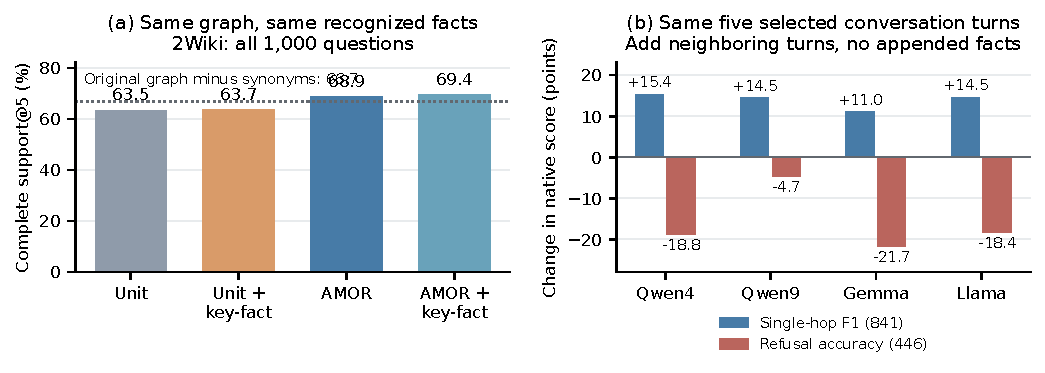
\includegraphics[width=\textwidth]{figures/memory_operations.pdf}
\caption{\textbf{Controlled changes in memory use.} Left: complete annotated support on all 1,000 2Wiki questions. ``Key-fact'' transfers CatRAG's released weighting operator; it is not the full CatRAG system. Graph connections and query initialization are identical across bars. The dotted line is a separate original-graph pruning control. Right: adding neighboring turns to the same five central turns, without appended facts, helps answerable questions but harms refusal. Each reader is shown separately.}
\label{fig:memory-operations}
\end{figure*}

\subsection{Source Context Can Both Repair and Reverse Consolidation}

\paragraph{A discarded assertion can return through its original text.}
Fact selection and source presentation are separate operations in AMOR.
In FC-SH, consolidation retains the updated UK assertion about \emph{Witches of East End}, but both the old USA source and the new UK source enter the answer context.
Even with the UK source first, all four readers fail without appended facts.
Removing only the appended UK assertion from full AMOR also flips all four answers; the five texts and nine other facts remain fixed.
Replacing it with the extracted USA assertion fails, while restoration recovers all four answers.
Across all 100 questions, allowing all extracted facts into augmentation instead of retained facts costs 15/14/15/17 EM points at the same ten-fact budget.
The retained assertion does work beyond storing the correction: it governs the use of competing original texts.

\paragraph{The same return is useful when consolidation removed a historical event.}
LightMem documents erroneous deletion of related, noncontradictory history~\citep{fang2026lightmem}; AMOR also exhibits this failure.
For Nate's activity during Joanna's trip, OpenIE extracted the tournament win, but a later \emph{won} statement displaced it under AMOR's subject--relation retention rule.
The annotated reply remains ranked first and says only ``while you were winning.''
Its neighboring source identifies the event.
Removing that turn lowers F1 from 80/80/75/80 to 0/0/0/40; restoring the original extracted fact to the five central turns gives 80/88.9/100/100.
Source expansion here repairs a loss introduced by construction itself.

Across answerable LoCoMo categories, 104 of 2,345 resolvable question/support-turn occurrences lose every extracted fact and become isolated in the graph.
Central turns include 23 of these occurrences; their neighbors raise coverage to 55.
Expansion can expose information removed by consolidation, which helps historical questions but can also reintroduce superseded assertions.
This explains why source preservation and retained-fact presentation serve different purposes within the same memory.

\begin{table*}[t]
\centering
\small
\setlength{\tabcolsep}{4pt}
\begin{tabular}{p{.18\textwidth}p{.32\textwidth}p{.29\textwidth}p{.16\textwidth}}
\toprule
Question / data & Verified source evidence & Controlled change or comparison & Native outcome \\
\midrule
Older film director?\newline 2Wiki & \emph{God's Gift to Women}: Michael Curtiz; Curtiz born 1886; Edith Carlmar born 1911. & Only Curtiz--biography weight $26\to1$; restore $1\to26$ on unit graph. & Complete support $4/4\to3/4\to4/4$. \\
\addlinespace[2pt]
\emph{Dubliners}' author's death place?\newline FC-MH & Update 7516: George Eliot; source 13652: London. & Substitute older accepted authorship. Correction remains; London source disappears. & Correct readers $4/4\to0/4\to4/4$ on restoration. \\
\addlinespace[2pt]
\emph{Witches of East End}'s country?\newline FC-SH & Old source 1836: USA; newer source 4787: UK. Both are selected. & Remove only appended UK assertion; preserve five texts and nine other facts. & Correct readers $4/4\to0/4\to4/4$ on restoration. \\
\addlinespace[2pt]
Kirton End's city population in 2001?\newline RULER MH-Doc & Distractor: another Kirton, 1,146 in 2011. Correct: Boston, 35,124 in 2001. & AMOR supplies the dated Boston source; HippoRAG~2 supplies the distractor. & AMOR $4/4$; all seven external baselines $0/4$ each. \\
\addlinespace[2pt]
Activity during Joanna's trip?\newline LoCoMo & D17:2: ``while you were winning''; D17:1: fourth video-game-tournament win. & Remove explanatory neighbor D17:1 from otherwise unchanged full context. & F1 $80/80/75/80\to0/0/0/40$. \\
\addlinespace[2pt]
Melanie's art-show inspiration?\newline LoCoMo & D9:16: \emph{Caroline}'s visit to an LGBTQ center inspired her. & Add neighbors and facts to central turns; readers adopt the other speaker's event. & Correct refusals $4/4\to0/4$. \\
\bottomrule
\end{tabular}
\caption{\textbf{Source-verified examples across four data origins.} FC assertions are benchmark counterfactuals. The 2Wiki fractions count support passages; other fractions count readers. RULER is a system comparison. The remaining rows state the intervened component. Full source text, predictions, and adverse outcomes accompany the section.}
\label{tab:memory-examples}
\end{table*}

\subsection{Recovery of Related Context Has an Answerability Cost}

The all-question LoCoMo experiment isolates this cost (Figure~\ref{fig:memory-operations}).
With central turns fixed and no appended facts, neighboring turns improve F1 on all 841 single-hop questions by 15.40/14.48/11.04/14.51 points, but reduce refusal accuracy on all 446 adversarial questions by 18.83/4.71/21.75/18.39 points.
LoCoMo already reports speaker confusion~\citep{maharana-etal-2024-evaluating}; this experiment attributes opposite effects to the same source-expansion operation.
In the Melanie example, removing Caroline's explanation restores refusal for three readers; the fourth remains wrong under every single-turn removal.

The documentary example exposes a related qualification requirement: both town and year must match.
Across all 100 MH-Doc questions, recommendation corrects 18/16/15/21 answers and introduces 5/3/6/6 errors, giving net EM gains of 13/13/9/15 points.
SH-Doc gains are 9/11/10/8 points; overall LoCoMo scores instead decrease slightly for the two Qwen readers.
Additional context helps when it completes the requested association, but can hurt when it supplies a plausible event outside the requested person's history.
AMOR's gains depend on both constructing useful associations and preserving which assertion or event the question permits the reader to use.
